\documentclass[tikz,border=4pt]{standalone}
% Shared style for MultiMM figures (white background, logo palette)
\usepackage{tikz,pgfplots,amsmath}
\pgfplotsset{compat=1.16}
\usetikzlibrary{arrows.meta,calc,decorations.pathreplacing,positioning,backgrounds}
\definecolor{indigo}{HTML}{3B37A0}
\definecolor{violet}{HTML}{6A3AA8}
\definecolor{crimson}{HTML}{B5406C}
\definecolor{gold}{HTML}{E9A62C}
\definecolor{golddark}{HTML}{B9791A}
\definecolor{grey}{HTML}{8A8AA0}
\definecolor{lightgrey}{HTML}{E4E4EE}
\tikzset{
  bead/.style={circle,draw=#1!80!black,fill=#1!35,line width=0.5pt,minimum size=9pt,inner sep=0pt},
  bead/.default=indigo,
  lab/.style={font=\small},
}
\pgfplotsset{
  every axis/.append style={
    width=9.5cm,height=6.3cm,axis lines=left,line width=0.5pt,
    grid=major,grid style={draw=lightgrey,line width=0.3pt},
    tick label style={font=\small},label style={font=\normalsize},
    legend style={font=\footnotesize,draw=none,fill=white,fill opacity=0.8,text opacity=1},
    legend cell align=left,
  },
  every axis plot/.append style={line width=1.2pt,smooth},
}

\begin{document}
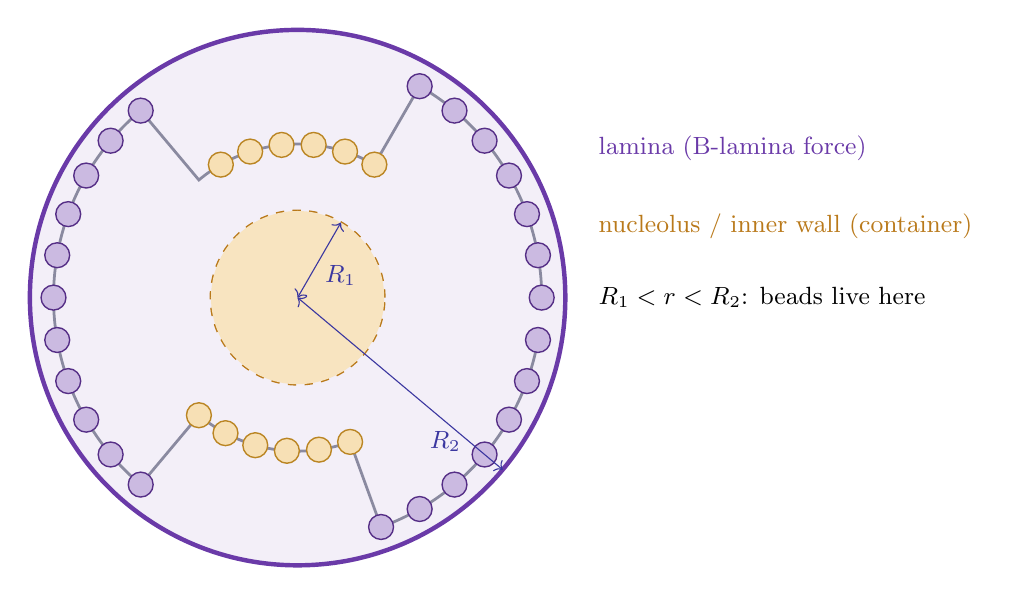
\begin{tikzpicture}
\def\Rb{3.4} \def\Ra{1.1}
\fill[violet!8] (0,0) circle (\Rb);
\draw[violet,line width=1.6pt] (0,0) circle (\Rb);
\draw[golddark,line width=1pt,dashed] (0,0) circle (\Ra);
\fill[gold!30] (0,0) circle (\Ra);
% one chromosome as a chain: B segments hug the lamina, A segments stay inside
\draw[grey,line width=1pt] (0:3.1) arc (0:60:3.1) -- (60:1.95) arc (60:130:1.95) -- (130:3.1)
  arc (130:230:3.1) -- (230:1.95) arc (230:290:1.95) -- (290:3.1) arc (290:350:3.1);
\foreach \a in {0,10,...,60}{\node[bead=violet] at (\a:3.1) {};}
\foreach \a in {130,140,...,230}{\node[bead=violet] at (\a:3.1) {};}
\foreach \a in {290,300,...,350}{\node[bead=violet] at (\a:3.1) {};}
\foreach \a in {60,72,...,130}{\node[bead=gold] at (\a:1.95) {};}
\foreach \a in {230,242,...,290}{\node[bead=gold] at (\a:1.95) {};}
\draw[<->,indigo] (0,0)--(60:1.1) node[midway,below right=-2pt,lab] {$R_1$};
\draw[<->,indigo] (0,0)--(-40:3.4) node[pos=0.72,below,lab] {$R_2$};
\node[lab,violet,anchor=west] at (3.7,1.9) {lamina (B-lamina force)};
\node[lab,golddark,anchor=west] at (3.7,0.9) {nucleolus / inner wall (container)};
\node[lab,anchor=west] at (3.7,0) {$R_1<r<R_2$: beads live here};
\end{tikzpicture}
\end{document}
